\section{SurveyReport Klassenreferenz}
\label{classSurveyReport}\index{SurveyReport@{SurveyReport}}
Klassendiagramm für SurveyReport::\begin{figure}[H]
\begin{center}
\leavevmode
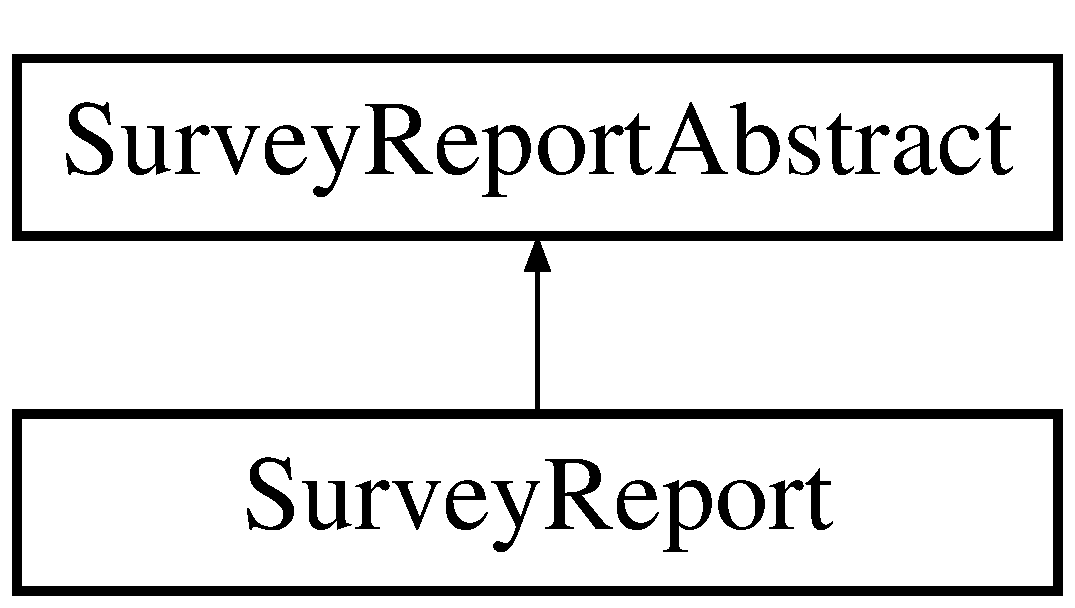
\includegraphics[height=2cm]{classSurveyReport}
\end{center}
\end{figure}
\subsection*{Öffentliche Methoden}
\begin{CompactItemize}
\item 
{\bf SurveyReport} (\$surveyID=null)
\item 
{\bf getSurveyTypeId} ()
\end{CompactItemize}
\subsection*{Öffentliche Attribute}
\begin{CompactItemize}
\item 
{\bf \$surveyTypeId}
\end{CompactItemize}


\subsection{Ausführliche Beschreibung}


Definiert in Zeile 10 der Datei class.SurveyReport.php.

\subsection{Dokumentation der Elementfunktionen}
\index{SurveyReport@{SurveyReport}!SurveyReport@{SurveyReport}}
\index{SurveyReport@{SurveyReport}!SurveyReport@{SurveyReport}}
\subsubsection{\setlength{\rightskip}{0pt plus 5cm}SurveyReport.SurveyReport (\$ {\em surveyID} = {\tt null})}\label{classSurveyReport_2fac5bc3ac1d78ee6e4d9f7be7bc5562}




Definiert in Zeile 13 der Datei class.SurveyReport.php.

Benutzt \$surveyObj und SurveyReportAbstract.\_\-loadDataBySurveyId().\index{SurveyReport@{SurveyReport}!getSurveyTypeId@{getSurveyTypeId}}
\index{getSurveyTypeId@{getSurveyTypeId}!SurveyReport@{SurveyReport}}
\subsubsection{\setlength{\rightskip}{0pt plus 5cm}SurveyReport.getSurveyTypeId ()}\label{classSurveyReport_e607b33b228b1b449c7cf42e8415e313}




Definiert in Zeile 59 der Datei class.SurveyReport.php.

\subsection{Dokumentation der Datenelemente}
\index{SurveyReport@{SurveyReport}!\$surveyTypeId@{\$surveyTypeId}}
\index{\$surveyTypeId@{\$surveyTypeId}!SurveyReport@{SurveyReport}}
\subsubsection{\setlength{\rightskip}{0pt plus 5cm}SurveyReport.\$surveyTypeId}\label{classSurveyReport_8afa69a6b9d08fe6b916dd68269900c9}




Definiert in Zeile 11 der Datei class.SurveyReport.php.

Die Dokumentation für diese Klasse wurde erzeugt aufgrund der Datei:\begin{CompactItemize}
\item 
{\bf class.SurveyReport.php}\end{CompactItemize}
